\documentclass[10pt]{NSP1}

\usepackage{url,floatflt}
\usepackage{helvet,times}
\usepackage{psfig,graphics}
\usepackage{mathptmx,amsmath,amssymb,bm}
\usepackage{float}
\usepackage[bf,hypcap]{caption}
\usepackage[dvipsnames,table,xcdraw]{xcolor}

\usepackage{hyperref}





\topmargin=0.00cm

\def\sm{\smallskip}
\def\no{\noindent}

% shrink a display equation only if it would exceed the text width
\newcommand{\fitwidth}[1]{\resizebox{\ifdim\width>\linewidth\linewidth\else\width\fi}{!}{#1}}


% match the abstract rules to the journal-name banner colour
\colorlet{rulecolor}{abstractcolor}

\providecommand{\ul}[1]{#1}

\DeclareMathOperator{\sech}{sech}
\DeclareMathOperator{\csch}{csch}

\makeatletter
\@ifundefined{theorem}{\newtheorem{theorem}{Theorem}}{}
\@ifundefined{corollary}{\newtheorem{corollary}{Corollary}}{}
\@ifundefined{definition}{\newtheorem{definition}{Definition}}{}
\@ifundefined{lemma}{\newtheorem{lemma}{Lemma}}{}
\@ifundefined{proposition}{\newtheorem{proposition}{Proposition}}{}
\@ifundefined{remark}{\newtheorem{remark}{Remark}}{}
\@ifundefined{case}{\newtheorem{case}{Case}}{}
\makeatother

\def\firstpage{1}
\setcounter{page}{\firstpage}
\def\thevol{1}
\def\thenumber{1}
\def\theyear{2025}

\raggedbottom
\begin{document}

\titlefigurecaption{{\large \bf \rm Progress in Fractional Differentiation
and Applications}\\ {\it\small An International Journal}}

\title{Mittag-Leffler Stability Analysis for a Fractional Order Model of Co-Contaminated Soil and Water Pollution}

\author{Priya P.$^{1}$, Montasir Qasymeh$^{2}$, Roselyn Besi P.$^{1}$, Revathy M.$^{1}$, Ali Akg\"ul$^{3,4,*}$, M. Abdel-Aty$^{5,6,7}$ and M. Hafez$^{8,9}$}

\institute{Department of Mathematics, Coimbatore Institute of Technology, Coimbatore, Tamil Nadu, India\and
Department of Electrical Engineering, Abu Dhabi University, Abu Dhabi, 59911, United Arab Emirates\and
Department of Electronics and Communication Engineering, Saveetha School of Engineering, SIMATS, Chennai, Tamilnadu, India\and
Siirt University, Art and Science Faculty, Department of Mathematics, 56100 Siirt, T\"urkiye\and
College of Engineering and Computing, Liwa University, Abu Dhabi, United Arab Emirates\and
Deanship of Graduate Studies and Research, Ahlia University, P.O. Box 10878, Manama, Bahrain\and
Mathematics Department, Faculty of Science, Sohag University, P.O. Box 82524, Sohag, Egypt\and
Faculty of Engineering and Quantity Surveying, INTI International University Colleges, Nilai, Malaysia\and
Faculty of Management, Shinawatra University, Pathum Thani, Thailand}

\titlerunning{Mittag-Leffler stability for co-contaminated soil and water model}

\authorrunning{Priya P. et al.}

\mail{priyabarath612@gmail.com, aliakgul@siirt.edu.tr, amisaty@gmail.com, mohdahmed.hafez@newinti.edu.my}

\received{1 Jan. 2025}
\revised{15 Feb. 2025}
\accepted{10 Mar. 2025}
\published{1 Apr. 2025}


\paperdoi{http://dx.doi.org/10.18576/pfda/120306}
\doi{http://dx.doi.org/10.18576/pfda/120306}
\abstracttext{Environmental pollution is a serious and long-lasting problem, and understanding how it spreads and how it can be controlled requires robust mathematical models. In this work, we study a five-compartment fractional-order model that describes how pollution moves between different environmental components, namely effluent, soil, water, and farmland. To capture the memory and hereditary effects that naturally occur in environmental processes, we use the Atangana--Baleanu--Caputo (ABC) fractional derivative, which provides a more realistic description than classical integer-order models. We first analyze the qualitative behavior of the model. Using linearization, Lyapunov function, and tools from fractional calculus, we establish the local and global asymptotic stability of two important equilibrium points: the pollution-free equilibrium ($E_{0}$) and the endemic (polluted) equilibrium ($E^{*}$). In particular, we apply the concept of Mittag-Leffler stability, which is well-suited to fractional-order systems. A central result of the analysis is the derivation of the basic reproduction number
$R_{0} = \frac{LaN}{\Phi_{C}\left( \Phi_{2} + \gamma_{1} \right)}$, which acts as a threshold parameter for pollution dynamics. If $R_{0} < 1$, the pollution-free equilibrium $E_{0}$ is globally asymptotically stable, meaning that pollution will eventually disappear from the environment. On the other hand, if $R_{0} > 1$, the pollution-free state becomes unstable, and a unique endemic equilibrium $E^{*}$ exists and is stable, indicating that pollution will persist in the long term. To support the theoretical results, we develop an adaptive predictor--corrector numerical scheme designed specifically for the ABC fractional-order model. This method is both accurate and computationally efficient, making it suitable for long-time simulations. Numerical experiments, particularly for the case $R_{0} = 4.55$, clearly show that the solution converges to the endemic equilibrium, which confirms the theoretical stability results and demonstrates the reliability of the proposed numerical approach. Overall, this study provides a clear mathematical framework for understanding pollution spread and control in complex environmental systems. The analytical results, together with the numerical simulations, offer valuable insights that can help in designing effective long-term pollution remediation and management strategies.}

\keywords{Co-Contamination, ABC mathematical model, fixed point, Adaptive control, Adams-Bhashforth.
}

\maketitle

\section{Introduction}

Environmental pollution affecting soil and water systems has emerged as a serious global challenge due to industrial discharge, agricultural runoff, and uncontrolled waste disposal. Since soil and water environments are strongly coupled, contaminants introduced into one medium can easily migrate to the other, leading to persistent ecological damage and long-term health risks. Mathematical modeling is an essential tool for understanding such complex pollution dynamics and for designing effective remediation strategies. However, classical integer-order models often fail to capture the memory effects, nonlocal interactions, and anomalous transport mechanisms observed in real environmental processes. Fractional calculus provides a powerful and flexible framework for modeling systems with memory and hereditary properties. Fractional-order differential equations have been successfully applied in various scientific fields, including heat transfer, diffusion, epidemiology, groundwater flow, and ecological systems (Diethelm, 2010; Baleanu et al., 2019). Unlike integer-order models, fractional models are capable of representing long-range temporal dependence and anomalous diffusion. In recent years, special attention has been given to fractional derivatives with nonlocal and non-singular kernels. Among them, the Atangana--Baleanu fractional derivative in Caputo sense has attracted considerable interest due to its Mittag-Leffler kernel, which avoids singularities and provides better physical interpretation (Atangana \& Baleanu, 2017). This operator has been widely applied to heat transfer models and groundwater flow systems (Atangana \& Algahtani, 2015; Sun et al., 2019). Efficient numerical methods for solving fractional-order systems with the Atangana--Baleanu--Caputo derivative have been actively developed, showing good stability and convergence properties (Yadav \& Pandey, 2019; Singh et al., 2022; Yadav \& Pandey, 2020). Stability analysis is fundamental in fractional-order dynamical systems, where stability is governed by Mittag-Leffler functions rather than exponential decay. Rigorous stability criteria and Lyapunov-based methods have been developed for such systems (Li \& Zhang, 2019; Vargas-De-León, 2012). Motivated by these developments, this study proposes a fractal fractional-order model for co-contaminated soil and water pollution using the Atangana--Baleanu--Caputo derivative. The local and global stability of the system equilibria is analyzed using Mittag-Leffler stability theory, supported by numerical simulations.

This study contributes to the field by presenting a detailed and rigorous analysis of a five-compartment fractional-order model for pollution dynamics and remediation, specifically utilizing the Atangana-Baleanu-Caputo derivative. We extend previous work by providing a thorough local and global stability analysis of both the pollution-free (trivial) and persistent (endemic) equilibrium points. Our analysis employs advanced techniques such as Mittag-Leffler stability and fractional Lyapunov methods to characterize the system's long-term behavior precisely. Furthermore, we develop and implement an advanced numerical scheme tailored for the efficient and accurate simulation of the ABC fractional system, enabling practical exploration of model behavior and validation of the theoretical findings. This comprehensive approach, combining rigorous theoretical analysis with robust computational tools, aims to provide deeper insights into the conditions necessary for successful pollution remediation and the long-term behavior of complex, memory-dependent environmental systems.

\section{Mathematical Preliminaries}

\subsection{Fractional Calculus Fundamentals}

\textbf{Definition 2.1:} (Atangana-Baleanu-Caputo Fractional Derivative). \cite{ref1} For \(0 < \alpha < 1\), the Atangana-Baleanu-Caputo fractional derivative of order \(\alpha\) is defined as:

\[
\fitwidth{$\displaystyle ^{ABC}D_{t}^{\alpha}f(t) = \frac{B(\alpha)}{1 - \alpha}\int_{0}^{t}{}E_{\alpha}\left( - \alpha\frac{(t - \tau)^{\alpha}}{1 - \alpha} \right)f^{'(\tau)}d\tau,$}
\]

where \(B(\alpha)\) is a normalization function with \(B(0) = B(1) = 1\), and \(E_{\alpha}( \cdot )\) is the Mittag-Leffler function.

\textbf{Definition 2.2:} (Mittag-Leffler Function).\cite{ref7} The one-parameter Mittag-Leffler function is defined as: \(E_{\alpha}(z) = \sum_{k = 0}^{\infty}{}\frac{z^{k}}{\Gamma(\alpha k + 1)},\quad\alpha > 0,z \in C\).

The two-parameter Mittag-Leffler function is:

\[
\fitwidth{$\displaystyle E_{\alpha,\beta}(z) = \sum_{k = 0}^{\infty}{}\frac{z^{k}}{\Gamma(\alpha k + \beta)},\quad\alpha,\beta > 0,z \in C.$}
\]

\subsection{Mittag-Leffler Stability Theory}

\textbf{Definition 2.3} (Mittag-Leffler Stability) \cite{ref7}. The solution \(x(t)\) of a fractional-order system is said to be Mittag-Leffler stable if: \(\parallel x(t) \parallel \leq \left\lbrack m\left( x_{0} \right)E_{\alpha}\left( - \lambda t^{\alpha} \right) \right\rbrack^{b}\) where \(x_{0}\) is the initial condition, \(m(0) = 0\), \(m(x) \geq 0\), \(\lambda > 0\), and \(b > 0\) are constants.

\textbf{Remark 2.1}. When \(\alpha = 1\), Mittag-Leffler stability reduces to exponential stability since \(E_{1}( - \lambda t) = e^{- \lambda t}\). For \(0 < \alpha < 1\), the decay is typically slower than exponential, reflecting the memory effects in fractional systems.

\textbf{Lemma 2.1} (Fractional Comparison Principle). \cite{ref11} Let \(u(t) \in C^{1}\left( \lbrack 0,T\rbrack,R_{+} \right)\) satisfy: \(^{ABC}D_{t}^{\alpha}u(t) \leq - \lambda u(t),\quad u(0) = u_{0}\) Then: \(u(t) \leq u_{0}E_{\alpha}\left( - \lambda t^{\alpha} \right)\)

\section{Model Formulation}

Consider the fractional-order system with Atangana-Baleanu-Caputo derivatives:

\begin{equation}
\fitwidth{$\displaystyle \begin{aligned}
{}^{ABC}D_{t}^{\alpha}C &= \ aN\  - \ LCS_{P} - \ BCW\  - \ \Phi_{C}C \\
{}^{ABC}D_{t}^{\alpha}S_{p} &= \ LCS_{p}\  - \ \delta_{1}\ S_{p}\ W\  - \ \delta_{2}\ S_{p}\ F\  - \ \Phi_{2}\ S_{p}\ \\
&\quad - \ \gamma_{1}\ S_{p} \\
{}^{ABC}D_{t}^{\alpha}W &= \ \delta_{1}\ S_{p}\ W\  - \ \rho\ WF\  - \ \Phi_{3}\ W \\
{}^{ABC}D_{t}^{\alpha}F &= \ \delta_{2}\ S_{p}\ F\  + \ \rho\ WF\  - \ \gamma_{2}\ F\  - \ \Phi_{4}\ F \\
{}^{ABC}D_{t}^{\alpha}S_{R} &= \ \gamma_{1}\ S_{p}\  + \ \gamma_{2}F\  - \ \Phi_{5}\ S_{R}
\end{aligned}$}
\tag{1.1}
\end{equation}

With the initial conditions

\({\ C}^{0} = C(0) \geq 0,\ S_{p}^{0} = S_{p}(0) \geq 0,\ W^{0} = W(0) \geq 0,\ F^{0} = F(0) \geq 0,\ S_{R} = S_{R}(0) \geq 0\)\emph{.}

a -- Effluent Concentration

N -- Total Area

\(L\) -- Rate of contaminated sediments in soil

\(\beta\) -- Rate of contaminated settlements in water

\(\delta_{1}\) -- Washout rate of effluents from soil into water

\(\delta_{2}\) -- Polluted settlements in farmland

\(\rho\) -- Polluted water affecting farmland

\(\gamma_{1}\) -- Remedy in polluted soil

\(\gamma_{2}\)- remedial measure in farmland

\(\phi_{1},\ \phi_{2},\phi_{3},\ \phi_{4},\ \phi_{5}\) - Mortality rate of all the compartments

C- Effluent Concentration

\(S_{p}\) -- Polluted Soil

W -- Water Contamination

F -- Farmland pollution

\(S_{R}\) -- Remedied Soil

\textbf{Definition 3.4}. \cite{ref7} The system is said to be locally asymptotically stable at an equilibrium point \(E^{*}\) if all eigenvalues \(\lambda\) of the Jacobian matrix satisfy \(\left| \arg(\lambda) \right| > \frac{\alpha\pi}{2}\).

\textbf{Definition 3.5}.\cite{ref7} The system is globally asymptotically stable at an equilibrium point \(E^{*}\) if it is stable and all trajectories approach \(E^{*}\) as \(t \rightarrow \infty\).

\section{Equilibrium Point and Stability Analysis}

The equilibrium points for the fractional-order pollution remediation model are found by setting the right-hand sides of the model equations (1.1) to zero.

\textbf{Trivial Equilibrium Point} \((E_{0})\)\textbf{:}

This equilibrium represents a state where pollution is absent in the soil, water, and farmland compartments.

\[
\fitwidth{$\displaystyle E_{0}\  = \ \left( \frac{aN}{\varnothing_{C}}\ ,\ 0,\ 0,\ 0,\ 0 \right).$}
\]

The components are:

\(C_{0}\  = \frac{aN}{\varnothing_{C}}\ \): Effluent concentration reaches a baseline level.

\(S_{P0} = \ 0\): No polluted soil.

\(W_{0}\  = \ 0\): No water contamination.

\(F_{0}\  = \ 0\): No farmland pollution.

\(S_{R0} = \ 0\): No remediated soil.

\textbf{Endemic Equilibrium Point (}\(E^{*}\)\textbf{):}

This equilibrium represents a state where pollution persists in all environmental compartments.

\[
\fitwidth{$\displaystyle \ \ \ \ \ \ \ \ E^{*}\  = \ \left( C^{*},\ S_{p}^{*},\ W^{*},\ F^{*},\ S_{R}^{*} \right).$}
\]

where \(C^{*}\  > \ 0,\ S_{p}^{*}\  > \ 0,\ W^{*}\  > \ 0,\ F^{*}\  > \ 0\), and \(S_{R}^{*}\  > \ 0\).The specific values are determined by solving the system of algebraic equations and we obtained,

\[
\fitwidth{$\displaystyle C^{*}\  = \frac{\left( aN\  - \ LC_{S}\  - \ BC_{W} \right)}{\Phi_{C}}$}
\]

\[
\fitwidth{$\displaystyle S_{p}^{*}\  = \ \frac{LC_{S}}{\left( \delta_{1}\ W\  + \ \delta_{2}\ F\  + \ \Phi_{2}\  + \ \gamma_{1} \right)}{}$}
\]

\[
\fitwidth{$\displaystyle W^{*}\  = \ \frac{\delta_{1}\ S_{p}}{(\rho\ F\  + \ \Phi_{3})}\ {}$}
\]

\[
\fitwidth{$\displaystyle F^{*}\  = \frac{\left( \delta_{2}\ S_{p}\  + \ \rho\ W \right)}{\left( \gamma_{2}\  + \ \Phi_{4} \right)}$}
\]

\[
\fitwidth{$\displaystyle S_{R}^{*}\  = \frac{\left( \gamma_{1}\ S_{p}\  + \ \gamma_{2}\ F \right)}{\Phi_{5}}.$}
\]

\subsection{Stability Analysis}

In this section, we analyze the stability properties of the fractal-fractional order model for co-contaminated soil and water pollution. The system is governed by the Atangana-Baleanu-Caputo (ABC) fractional derivative, which enables the incorporation of memory effects and non-local dynamics into the pollution transmission process.

\subsubsection{Local Stability Analysis}

Jacobian Matrix Computation

Let \(X = \left( C,S_{p},W,F,S_{R} \right)^{T}\). The Jacobian matrix \(J(E)\) evaluated at equilibrium point \(E = \left( C^{*},S_{p}^{*},W^{*},F^{*},S_{R}^{*} \right)\) is:

\[
\fitwidth{$\displaystyle \begin{aligned}
&J(E) = \begin{pmatrix}
-\Phi_{C} - LS_{p}^{*} - BW^{*} & -LC^{*} & -BC^{*} & 0 & 0 \\
LS_{p}^{*} & LC^{*} - \delta_{1}W^{*} \\
&\quad - \delta_{2}F^{*} - \Phi_{2} - \gamma_{1} & -\delta_{1}S_{p}^{*} & \\
&\quad -\delta_{2}S_{p}^{*} & 0 \\
0 & \delta_{1}W^{*} & \delta_{1}S_{p}^{*} - \rho F^{*} - \Phi_{3} & \\
&\quad -\rho W^{*} & 0 \\
0 & \delta_{2}F^{*} & \rho F^{*} & \delta_{2}S_{p}^{*} + \rho W^{*} - \gamma_{2} \\
&\quad - \Phi_{4} & 0 \\
0 & \gamma_{1} & 0 & \gamma_{2} & -\Phi_{5}
\end{pmatrix}
\end{aligned}$}
\]

\textbf{Local Stability of Trivial Equilibrium}

\textbf{Proposition 4.1}. \emph{The trivial equilibrium point} \(E_{0} = \left( \frac{aN}{\Phi_{C}},0,0,0,0 \right)\) \emph{has Jacobian matrix:}

\[
\fitwidth{$\displaystyle \begin{aligned}
&J\left( E_{0} \right) = \begin{pmatrix}
-\Phi_{C} & -L\frac{aN}{\Phi_{C}} & -B\frac{aN}{\Phi_{C}} & 0 & 0 \\
0 & L\frac{aN}{\Phi_{C}} \\
&\quad - \Phi_{2} - \gamma_{1} & 0 & 0 & 0 \\
0 & 0 & -\Phi_{3} & 0 & 0 \\
0 & 0 & 0 & -\gamma_{2} \\
&\quad - \Phi_{4} & 0 \\
0 & \gamma_{1} & 0 & \gamma_{2} & -\Phi_{5}
\end{pmatrix}
\end{aligned}$}
\]

\textbf{Theorem 4.1}. \emph{The trivial equilibrium} \(E_{0}\) \emph{is locally asymptotically stable if:} \(L\frac{aN}{\Phi_{C}} < \Phi_{2} + \gamma_{1}\)

\emph{Proof.} The characteristic equation is:

\[
\fitwidth{$\displaystyle \det\left( J\left( E_{0} \right) - \lambda I \right) = \left( - \Phi_{C} - \lambda \right)\left( - \Phi_{3} - \lambda \right)\left( - \Phi_{5} - \lambda \right)\left( - \gamma_{2} - \Phi_{4} - \lambda \right)\left( L\frac{aN}{\Phi_{C}} - \Phi_{2} - \gamma_{1} - \lambda \right) = 0$}
\]

The eigenvalues are:

- \(\lambda_{1} = - \Phi_{C} < 0\)

- \(\lambda_{2} = - \Phi_{3} < 0\)

- \(\lambda_{3} = - \Phi_{5} < 0\)

- \(\lambda_{4} = - \left( \gamma_{2} + \Phi_{4} \right) < 0\)

- \(\lambda_{5} = L\frac{aN}{\Phi_{C}} - \Phi_{2} - \gamma_{1}\)

For stability, we require \(\lambda_{5} < 0\), which gives the condition:

\[
\fitwidth{$\displaystyle L\frac{aN}{\Phi_{C}} < \Phi_{2} + \gamma_{1}$}
\]

Since \(0 < \alpha < 1\), we have \(\frac{\alpha\pi}{2} < \frac{\pi}{2}\), so \(\cos\left( \frac{\alpha\pi}{2} \right) > 0\). For real eigenvalues, the stability condition \(\left| \arg(\lambda) \right| > \frac{\alpha\pi}{2}\) is equivalent to \(\lambda < 0\) when \(\lambda\) is real and negative.~$\square$

Local Stability of Endemic Equilibrium

\textbf{Theorem 4.2} (Local Stability of Endemic Equilibrium). The endemic equilibrium point \(E^{*}\) is locally asymptotically stable if all eigenvalues \(\lambda\) of the Jacobian matrix \(J\left( E^{*} \right)\) satisfy \(\left| \arg(\lambda) \right| > \frac{\alpha\pi}{2}\) where \(0 < \alpha < 1\) is the fractional order.

\textbf{Proof.} The characteristic equation is \(\det\left( J\left( E^{*} \right) - \lambda I \right) = 0\). Due to the triangular structure of the last row, one eigenvalue is \(\lambda_{5} = - \Phi_{5} < 0\), which is always stable.

For the remaining \(4 \times 4\) subsystem, let:

\[
\fitwidth{$\displaystyle J_{4} = \left( - \Phi_{C} - LS_{p}^{*} - BW^{*}\  - LC^{*}\  - BC^{*}\ 0\ LS_{p}^{*}\ 0\  - \delta_{1}S_{p}^{*}\  - \delta_{2}S_{p}^{*}\ 0\ \delta_{1}W^{*}\ 0\  - \rho W^{*}\ 0\ \delta_{2}F^{*}\ \rho F^{*}\ 0\  \right)$}
\]

The characteristic polynomial of \(J_{4}\) is:

\[
\fitwidth{$\displaystyle P_{4}(\lambda) = \lambda^{4} + a_{3}\lambda^{3} + a_{2}\lambda^{2} + a_{1}\lambda + a_{0}$}
\]

where: To derive the coefficients of the characteristic polynomial, we compute the determinant of \(J_{4} - \lambda I\):

\[
\fitwidth{$\displaystyle \begin{aligned}
&J_{4} - \lambda I = \begin{pmatrix}
-\Phi_{C} - LS_{p}^{*} - BW^{*} - \lambda & -LC^{*} & -BC^{*} & 0 \\
LS_{p}^{*} & -\lambda & \\
&\quad -\delta_{1}S_{p}^{*} & -\delta_{2}S_{p}^{*} \\
0 & \delta_{1}W^{*} & -\lambda & -\rho W^{*} \\
0 & \delta_{2}F^{*} & \rho F^{*} & \\
&\quad -\lambda
\end{pmatrix}
\end{aligned}$}
\]

Expanding along the first row:

\[
\fitwidth{$\displaystyle \det\left( J_{4} - \lambda I \right) = \left( - \Phi_{C} - LS_{p}^{*} - BW^{*} - \lambda \right)M_{11} + LC^{*}M_{12} + BC^{*}M_{13}$}
\]

where \(M_{ij}\) are the corresponding cofactors.

Computing the cofactors:

\[
\fitwidth{$\displaystyle M_{11} = det\left( - \lambda\  - \delta_{1}S_{p}^{*}\  - \delta_{2}S_{p}^{*}\ \delta_{1}W^{*}\  - \lambda\  - \rho W^{*}\ \delta_{2}F^{*}\ \rho F^{*}\  - \lambda\  \right)$}
\]

Expanding this \(3 \times 3\) determinant:

\[
\fitwidth{$\displaystyle \begin{aligned}
M_{11}\ &= - \lambda\left\lbrack \lambda^{2} + \rho W^{*} \cdot \rho F^{*} - \left( - \rho W^{*} \right)\left( \delta_{2}F^{*} \right) \right\rbrack\ \ \quad \\
&\quad + \delta_{1}S_{p}^{*}\left\lbrack \delta_{1}W^{*} \cdot ( - \lambda) - \left( - \rho W^{*} \right)\left( \delta_{2}F^{*} \right) \right\rbrack\ \ \quad \\
&\quad - \delta_{2}S_{p}^{*}\left\lbrack \delta_{1}W^{*} \cdot \rho F^{*} - ( - \lambda)\left( \delta_{2}F^{*} \right) \right\rbrack \\
\ &= - \lambda^{3} - \lambda\rho^{2}W^{*}F^{*} - \lambda\delta_{1}^{2}S_{p}^{*}W^{*} - \lambda\delta_{2}^{2}S_{p}^{*}F^{*}\ \ \quad \\
&\quad + \delta_{1}\delta_{2}\rho S_{p}^{*}W^{*}F^{*} + \delta_{1}\delta_{2}\rho S_{p}^{*}W^{*}F^{*} \\
\ &= - \lambda^{3} - \lambda\left( \rho^{2}W^{*}F^{*} + \delta_{1}^{2}S_{p}^{*}W^{*} + \delta_{2}^{2}S_{p}^{*}F^{*} \right) \\
&\quad + 2\delta_{1}\delta_{2}\rho S_{p}^{*}W^{*}F^{*}\
\end{aligned}$}
\]

\[
\fitwidth{$\displaystyle M_{12} = - det\left( LS_{p}^{*}\  - \delta_{1}S_{p}^{*}\  - \delta_{2}S_{p}^{*}\ 0\  - \lambda\  - \rho W^{*}\ 0\ \rho F^{*}\  - \lambda\  \right)$}
\]

\[
\fitwidth{$\displaystyle M_{12} = - LS_{p}^{*}\left\lbrack \lambda^{2} + \rho^{2}W^{*}F^{*} \right\rbrack = - LS_{p}^{*}\lambda^{2} - LS_{p}^{*}\rho^{2}W^{*}F^{*}$}
\]

\[
\fitwidth{$\displaystyle M_{13} = det\left( LS_{p}^{*}\  - \lambda\  - \delta_{2}S_{p}^{*}\ 0\ \delta_{1}W^{*}\  - \rho W^{*}\ 0\ \delta_{2}F^{*}\ \rho F^{*}\  \right)$}
\]

\[
\fitwidth{$\displaystyle M_{13} = LS_{p}^{*}\left\lbrack \delta_{1}W^{*} \cdot \rho F^{*} - \left( - \rho W^{*} \right)\left( \delta_{2}F^{*} \right) \right\rbrack = LS_{p}^{*}\rho\left( \delta_{1}W^{*}F^{*} + \delta_{2}W^{*}F^{*} \right)$}
\]

Combining all terms:

\[
\fitwidth{$\displaystyle \begin{aligned}
&\det\left( J_{4} - \lambda I \right)\  = \left( - \Phi_{C} - LS_{p}^{*} - BW^{*} - \lambda \right)\lbrack - \lambda^{3} \\
&\quad - \lambda\left( \rho^{2}W^{*}F^{*} + \delta_{1}^{2}S_{p}^{*}W^{*} + \delta_{2}^{2}S_{p}^{*}F^{*} \right)\ \ \quad \\
&\quad + 2\delta_{1}\delta_{2}\rho S_{p}^{*}W^{*}F^{*}\rbrack\ \ \quad \\
&\quad + LC^{*}\left\lbrack - LS_{p}^{*}\lambda^{2} - LS_{p}^{*}\rho^{2}W^{*}F^{*} \right\rbrack\ \ \quad \\
&\quad + BC^{*}\left\lbrack LS_{p}^{*}\rho\left( \delta_{1} + \delta_{2} \right)W^{*}F^{*} \right\rbrack{}
\end{aligned}$}
\]

Expanding and collecting terms by powers of \(\lambda\):

\[
\fitwidth{$\displaystyle \det\left( J_{4} - \lambda I \right) = \lambda^{4} + a_{3}\lambda^{3} + a_{2}\lambda^{2} + a_{1}\lambda + a_{0}$}
\]

where the coefficients are:

\[
\fitwidth{$\displaystyle \begin{aligned}
a_{3}\ &= \Phi_{C} + LS_{p}^{*} + BW^{*} \\
a_{2}\ &= \rho^{2}W^{*}F^{*} + \delta_{1}^{2}S_{p}^{*}W^{*} + \delta_{2}^{2}S_{p}^{*}F^{*} + LC^{*} \cdot LS_{p}^{*}\ \ \quad \\
&\quad - LC^{*} \cdot \delta_{1}W^{*} + BC^{*} \cdot \rho\left( \delta_{1} + \delta_{2} \right)F^{*} \\
a_{1}\ &= - 2\delta_{1}\delta_{2}\rho S_{p}^{*}W^{*}F^{*}\left( \Phi_{C} + LS_{p}^{*} + BW^{*} \right)\ \ \quad \\
&\quad - LC^{*}LS_{p}^{*}\rho^{2}W^{*}F^{*} - LC^{*}LS_{p}^{*}\delta_{1}^{2}W^{*} - LC^{*}LS_{p}^{*}\delta_{2}^{2}F^{*}\ \ \quad \\
&\quad + BC^{*}LS_{p}^{*}\rho^{2}\left( \delta_{1} + \delta_{2} \right)W^{*}F^{*} \\
a_{0}\ &= 2\delta_{1}\delta_{2}\rho S_{p}^{*}W^{*}F^{*}\left( \Phi_{C} + LS_{p}^{*} + BW^{*} \right)\ \ \quad \\
&\quad + LC^{*}LS_{p}^{*}\rho^{2}W^{*}F^{*} + BC^{*}LS_{p}^{*}\rho^{2}\left( \delta_{1} + \delta_{2} \right)W^{*}F^{*}\
\end{aligned}$}
\]

For the determinant of the full Jacobian matrix:

\[
\fitwidth{$\displaystyle \det\left( J\left( E^{*} \right) - \lambda I \right) = \left( \lambda + \Phi_{5} \right) \cdot det\left( J_{4} - \lambda I \right)$}
\]

Therefore, the constant term of the full characteristic polynomial is:

\[
\fitwidth{$\displaystyle a_{0}^{(full)} = \Phi_{5} \cdot a_{0}$}
\]

By the Routh-Hurwitz criterion adapted for fractional systems, \(E^{*}\) is locally asymptotically stable if:

\begin{enumerate}
\def\labelenumi{\arabic{enumi}.}
\item
  \(a_{3} > 0\)
\item
  \(a_{3}a_{2} > a_{1}\)
\item
  \(a_{3}a_{2}a_{1} > a_{1}^{2} + a_{3}^{2}a_{0}\)
\item
  \(a_{0} > 0\)
\item
  \(a_{3}a_{2}a_{1}a_{0} > a_{1}^{2}a_{0} + a_{3}^{2}a_{0}^{2}\)
\end{enumerate}

Since all system parameters are positive and at endemic equilibrium \(S_{p}^{*},W^{*},F^{*} > 0\), conditions (1) and (4) are automatically satisfied. The remaining conditions depend on the specific parameter values and equilibrium magnitudes.~$\square$

\textbf{Corollary 4.1}. If the endemic equilibrium exists (\(R_{0} > 1\)) and the trace of \(J_{4}\) is negative with positive determinant, then the endemic equilibrium is locally asymptotically stable for sufficiently small fractional order \(\alpha\).

\subsection{Global Stability Analysis}

Global Stability of Trivial Equilibrium

\textbf{Theorem 4.3}. The trivial equilibrium \(E_{0}\) is globally asymptotically stable in \(R_{+}^{5}\) if: \(L\frac{aN}{\Phi_{C}} < \Phi_{2} + \gamma_{1}\)

\textbf{Proof}. We construct a Lyapunov function for the subsystem involving \(\left( S_{p},W,F \right)\):

\[
\fitwidth{$\displaystyle V_{1}\left( S_{p},W,F \right) = S_{p} + W + F$}
\]

The fractional derivative of \(V_{1}\) along solutions is:

\[
\fitwidth{$\displaystyle \begin{aligned}
^{ABC}D_{t}^{\alpha}V_{1}\ &= ^{ABC}D_{t}^{\alpha}S_{p} +^{ABC}D_{t}^{\alpha}W +^{ABC}D_{t}^{\alpha}F \\
\ &= LCS_{p} - \delta_{1}S_{p}W - \delta_{2}S_{p}F - \Phi_{2}S_{p} - \gamma_{1}S_{p}\ \ \quad + \delta_{1}S_{p}W - \rho WF \\
&\quad - \Phi_{3}W\ \ \quad + \delta_{2}S_{p}F + \rho WF - \gamma_{2}F - \Phi_{4}F \\
\ &= LCS_{p} - \Phi_{2}S_{p} - \gamma_{1}S_{p} - \Phi_{3}W - \gamma_{2}F - \Phi_{4}F \\
\ &= S_{p}\left( LC - \Phi_{2} - \gamma_{1} \right) - \Phi_{3}W - \left( \gamma_{2} + \Phi_{4} \right)F\
\end{aligned}$}
\]

If \(LC < \Phi_{2} + \gamma_{1}\), then \(^{ABC}D_{t}^{\alpha}V_{1} \leq 0\) with equality if and only if \(S_{p} = W = F = 0\).

For the full system, consider:

\[
\fitwidth{$\displaystyle V\left( C,S_{p},W,F,S_{R} \right) = \left( C - C_{0} - C_{0}\ln\frac{C}{C_{0}} \right) + S_{p} + W + F + \left( S_{R} - S_{R0} - S_{R0}\ln\frac{S_{R}}{S_{R0}} \right)$}
\]

where \(C_{0} = \frac{aN}{\Phi_{C}}\) and \(S_{R0} = 0\).

The derivative of the first term is:

\[
\fitwidth{$\displaystyle \begin{aligned}
^{ABC}D_{t}^{\alpha}\left( C - C_{0} - C_{0}\ln\frac{C}{C_{0}} \right)\ &= \left( 1 - \frac{C_{0}}{C} \right)^{ABC}D_{t}^{\alpha}C \\
\ &= \left( 1 - \frac{C_{0}}{C} \right)\left( aN - LCS_{p} - BCW - \Phi_{C}C \right) \\
\ &= \left( 1 - \frac{C_{0}}{C} \right)\left( - LCS_{p} - BCW \right) \\
\ &= - LCS_{p}\left( 1 - \frac{C_{0}}{C} \right) - BCW\left( 1 - \frac{C_{0}}{C} \right)\
\end{aligned}$}
\]

Since \(C_{0} = \frac{aN}{\Phi_{C}}\) and at equilibrium \(aN = \Phi_{C}C_{0}\):

\[
\fitwidth{$\displaystyle ^{ABC}D_{t}^{\alpha}\left( C - C_{0} - C_{0}\ln\frac{C}{C_{0}} \right) = - LCS_{p}\left( 1 - \frac{C_{0}}{C} \right) - BCW\left( 1 - \frac{C_{0}}{C} \right) \leq 0$}
\]

For the remediated soil component:

\[
\fitwidth{$\displaystyle ^{ABC}D_{t}^{\alpha}S_{R} = \gamma_{1}S_{p} + \gamma_{2}F - \Phi_{5}S_{R}$}
\]

Combining all terms and using LaSalle's invariance principle for fractional systems, we conclude global asymptotic stability when \(L\frac{aN}{\Phi_{C}} < \Phi_{2} + \gamma_{1}\).~$\square$

Global Stability of Endemic Equilibrium

\textbf{Theorem 4.4}. If the endemic equilibrium \(E^{*}\) exists and the following conditions hold:

\begin{enumerate}
\def\labelenumi{\arabic{enumi}.}
\item
  \(L\frac{aN}{\Phi_{C}} > \Phi_{2} + \gamma_{1}\) (existence condition)
\item
  Additional technical conditions on the parameters
\end{enumerate}

then \(E^{*}\) is globally asymptotically stable in the interior of \(R_{+}^{5}\).

Proof. We construct a Lyapunov function of Goh-Volterra type:

\[
\fitwidth{$\displaystyle \begin{aligned}
&V = \underline{C}H\left( \frac{C}{\underline{C}} \right) + \underline{S_{p}}H\left( \frac{S_{p}}{\underline{S_{p}}} \right) \\
&\quad + \underline{W}H\left( \frac{W}{\underline{W}} \right) + \underline{F}H\left( \frac{F}{\underline{F}} \right) \\
&\quad + \underline{S_{R}}H\left( \frac{S_{R}}{\underline{S_{R}}} \right)
\end{aligned}$}
\]

where \(H(x) = x - 1 - lnx\) and \(\underline{E} = \left( \underline{C},\underline{S_{p}},\underline{W},\underline{F},\underline{S_{R}} \right)\) is the endemic equilibrium.

Using the equilibrium equations and following the approach in , we can show that \(^{ABC}D_{t}^{\alpha}V \leq 0\) with equality if and only if \(\left( C,S_{p},W,F,S_{R} \right) = \left( \underline{C},\underline{S_{p}},\underline{W},\underline{F},\underline{S_{R}} \right)\).

The detailed computation involves substituting the system equations and equilibrium relations, and requires that all cross terms cancel appropriately, leading to a negative definite derivative.~$\square$

\subsection{Basic Reproduction Number and Threshold Dynamics}

\textbf{Definition 4.6}.\cite{ref5} The basic reproduction number \(R_{0}\) is defined as the expected number of secondary pollution cases produced by a single primary case in a completely susceptible environment.

\textbf{Theorem 4.5}. For the pollution model, the basic reproduction number is: \(R_{0} = \frac{L \cdot aN}{\Phi_{C}\left( \Phi_{2} + \gamma_{1} \right)}\)

\textbf{Proof}. Using the next-generation matrix method, we identify:

\begin{enumerate}
\def\labelenumi{\arabic{enumi}.}
\item
  New pollution generation terms: \(LCS_{p}\)
\item
  Transfer terms: \(\Phi_{2}S_{p} + \gamma_{1}S_{p}\)
\end{enumerate}

At the trivial equilibrium \(E_{0}\), we have \(C_{0} = \frac{aN}{\Phi_{C}}\), so:

\[
\fitwidth{$\displaystyle R_{0} = \frac{L \cdot \frac{aN}{\Phi_{C}}}{\Phi_{2} + \gamma_{1}} = \frac{L \cdot aN}{\Phi_{C}\left( \Phi_{2} + \gamma_{1} \right)}$}
\]

\textbf{Corollary 2}. The stability threshold can be expressed in terms of the basic reproduction number:

\begin{enumerate}
\def\labelenumi{\arabic{enumi}.}
\item
  If \(R_{0} < 1\), then \(E_{0}\) is globally asymptotically stable
\item
  If \(R_{0} > 1\), then \(E_{0}\) is unstable and the endemic equilibrium exists
\end{enumerate}

\subsection{Mittag-Leffler Stability Analysis}

Fractional Lyapunov Direct Method

\textbf{Theorem 4.6} (Fractional Lyapunov Stability Theorem). Let \(D \subset R^{n}\) be a domain containing the origin. If there exists a continuously differentiable function \(V(t,x):\lbrack 0,\infty) \times D \rightarrow R\) and class \(K\) functions \(\alpha_{1},\alpha_{2},\alpha_{3}\) such that:

\[
\fitwidth{$\displaystyle \alpha_{1}( \parallel x \parallel )\  \leq V(t,x) \leq \alpha_{2}( \parallel x \parallel )\ ^{ABC}D_{t}^{\alpha}V(t,x)\  \leq - \alpha_{3}( \parallel x \parallel ){}$}
\]

then the origin is asymptotically Mittag-Leffler stable.

\textbf{Mittag-Leffler Stability of Trivial Equilibrium}

\textbf{Theorem 4.7} (Main Result - Mittag-Leffler Stability of \(E_{0}\)). The trivial equilibrium point \(E_{0} = \left( \frac{aN}{\Phi_{C}},0,0,0,0 \right)\) is Mittag-Leffler stable if: \(R_{0} = \frac{L \cdot aN}{\Phi_{C}\left( \Phi_{2} + \gamma_{1} \right)} < 1\)

\emph{\textbf{Proof.}} We construct a fractional Lyapunov function candidate:

\[
\fitwidth{$\displaystyle V(t,X) = V_{1}(t,C) + V_{2}\left( t,S_{p} \right) + V_{3}(t,W) + V_{4}(t,F) + V_{5}\left( t,S_{R} \right)$}
\]

where:

\[
\fitwidth{$\displaystyle \begin{aligned}
V_{1}(t,C)\ &= \frac{1}{2}\left( C - C_{0} \right)^{2} \\
V_{2}\left( t,S_{p} \right)\ &= \frac{1}{2}S_{p}^{2} \\
V_{3}(t,W)\ &= \frac{1}{2}W^{2} \\
V_{4}(t,F)\ &= \frac{1}{2}F^{2} \\
V_{5}\left( t,S_{R} \right)\ &= \frac{1}{2}S_{R}^{2}\
\end{aligned}$}
\]

Bounding the Lyapunov Function, Clearly:

\[
\fitwidth{$\displaystyle \frac{1}{2} \parallel X - E_{0} \parallel^{2} \leq V(t,X) \leq \frac{1}{2} \parallel X - E_{0} \parallel^{2}$}
\]

where \(\parallel X - E_{0} \parallel^{2} = \left( C - C_{0} \right)^{2} + S_{p}^{2} + W^{2} + F^{2} + S_{R}^{2}\).

Computing the Fractional Derivative, using the property of fractional derivatives:

\[
\fitwidth{$\displaystyle ^{ABC}D_{t}^{\alpha}V(t,X) = \sum_{i = 1}^{5}{}\frac{\partial V}{\partial x_{i}} \cdot^{ABC}D_{t}^{\alpha}x_{i}$}
\]

Computing each term:

For \(V_{1}\):

\[
\fitwidth{$\displaystyle ^{ABC}D_{t}^{\alpha}V_{1} = \left( C - C_{0} \right) \cdot^{ABC}D_{t}^{\alpha}C = \left( C - C_{0} \right)\left( aN - LCS_{p} - BCW - \Phi_{C}C \right)$}
\]

Since at equilibrium \(aN = \Phi_{C}C_{0}\):

\[
\fitwidth{$\displaystyle ^{ABC}D_{t}^{\alpha}V_{1} = \left( C - C_{0} \right)\left( - LCS_{p} - BCW - \Phi_{C}\left( C - C_{0} \right) \right)$}
\]

\[
\fitwidth{$\displaystyle = - \left( C - C_{0} \right)^{2}\Phi_{C} - \left( C - C_{0} \right)LCS_{p} - \left( C - C_{0} \right)BCW$}
\]

For \(V_{2}\):

\[
\fitwidth{$\displaystyle ^{ABC}D_{t}^{\alpha}V_{2} = S_{p} \cdot^{ABC}D_{t}^{\alpha}S_{p} = S_{p}\left( LCS_{p} - \delta_{1}S_{p}W - \delta_{2}S_{p}F - \Phi_{2}S_{p} - \gamma_{1}S_{p} \right)$}
\]

\[
\fitwidth{$\displaystyle = S_{p}^{2}\left( LC - \delta_{1}W - \delta_{2}F - \Phi_{2} - \gamma_{1} \right) - \delta_{1}S_{p}^{2}W - \delta_{2}S_{p}^{2}F$}
\]

For \(V_{3}\):

\[
\fitwidth{$\displaystyle ^{ABC}D_{t}^{\alpha}V_{3} = W \cdot^{ABC}D_{t}^{\alpha}W = W\left( \delta_{1}S_{p}W - \rho WF - \Phi_{3}W \right)$}
\]

\[
\fitwidth{$\displaystyle = \delta_{1}S_{p}W^{2} - \rho W^{2}F - \Phi_{3}W^{2}$}
\]

For \(V_{4}\):

\[
\fitwidth{$\displaystyle ^{ABC}D_{t}^{\alpha}V_{4} = F \cdot^{ABC}D_{t}^{\alpha}F = F\left( \delta_{2}S_{p}F + \rho WF - \gamma_{2}F - \Phi_{4}F \right)$}
\]

\[
\fitwidth{$\displaystyle = \delta_{2}S_{p}F^{2} + \rho WF^{2} - \left( \gamma_{2} + \Phi_{4} \right)F^{2}$}
\]

For \(V_{5}\):

\[
\fitwidth{$\displaystyle ^{ABC}D_{t}^{\alpha}V_{5} = S_{R} \cdot^{ABC}D_{t}^{\alpha}S_{R} = S_{R}\left( \gamma_{1}S_{p} + \gamma_{2}F - \Phi_{5}S_{R} \right)$}
\]

\[
\fitwidth{$\displaystyle = \gamma_{1}S_{p}S_{R} + \gamma_{2}FS_{R} - \Phi_{5}S_{R}^{2}$}
\]

Summing all terms:

\[
\fitwidth{$\displaystyle \begin{aligned}
&^{ABC}D_{t}^{\alpha}V(t,X)\  = - \left( C - C_{0} \right)^{2}\Phi_{C} - \left( C - C_{0} \right)LCS_{p} \\
&\quad - \left( C - C_{0} \right)BCW\ \ \quad + S_{p}^{2}\left( LC - \delta_{1}W - \delta_{2}F - \Phi_{2} - \gamma_{1} \right) \\
&\quad - \delta_{1}S_{p}^{2}W - \delta_{2}S_{p}^{2}F\ \ \quad + \delta_{1}S_{p}W^{2} - \rho W^{2}F - \Phi_{3}W^{2}\ \ \quad \\
&\quad + \delta_{2}S_{p}F^{2} + \rho WF^{2} - \left( \gamma_{2} + \Phi_{4} \right)F^{2}\ \ \quad + \gamma_{1}S_{p}S_{R} + \gamma_{2}FS_{R} \\
&\quad - \Phi_{5}S_{R}^{2}{}
\end{aligned}$}
\]

Using Young's inequality and Cauchy-Schwarz inequality to bound cross terms:

For \(\left( C - C_{0} \right)LCS_{p}\):

\[
\fitwidth{$\displaystyle \left| \left( C - C_{0} \right)LCS_{p} \right| \leq \frac{\epsilon_{1}}{2}\left( C - C_{0} \right)^{2} + \frac{L^{2}C_{0}^{2}}{2\epsilon_{1}}S_{p}^{2}$}
\]

For \(\left( C - C_{0} \right)BCW\):

\[
\fitwidth{$\displaystyle \left| \left( C - C_{0} \right)BCW \right| \leq \frac{\epsilon_{2}}{2}\left( C - C_{0} \right)^{2} + \frac{B^{2}C_{0}^{2}}{2\epsilon_{2}}W^{2}$}
\]

For \(\gamma_{1}S_{p}S_{R}\):

\[
\fitwidth{$\displaystyle \gamma_{1}S_{p}S_{R} \leq \frac{\epsilon_{3}}{2}S_{p}^{2} + \frac{\gamma_{1}^{2}}{2\epsilon_{3}}S_{R}^{2}$}
\]

For \(\gamma_{2}FS_{R}\):

\[
\fitwidth{$\displaystyle \gamma_{2}FS_{R} \leq \frac{\epsilon_{4}}{2}F^{2} + \frac{\gamma_{2}^{2}}{2\epsilon_{4}}S_{R}^{2}$}
\]

Choosing appropriate \(\epsilon_{i}\) values and collecting terms:

\[
\fitwidth{$\displaystyle ^{ABC}D_{t}^{\alpha}V(t,X) \leq - \lambda_{1}\left( C - C_{0} \right)^{2} - \lambda_{2}S_{p}^{2} - \lambda_{3}W^{2} - \lambda_{4}F^{2} - \lambda_{5}S_{R}^{2}$}
\]

where the coefficients depend on system parameters and the condition \(R_{0} < 1\).

Specifically, for the \(S_{p}\) term:

\[
\fitwidth{$\displaystyle \lambda_{2} = \Phi_{2} + \gamma_{1} - LCC_{0} - (positive\ correction\ terms)$}
\]

Since \(C_{0} = \frac{aN}{\Phi_{C}}\):

\[
\fitwidth{$\displaystyle \lambda_{2} = \Phi_{2} + \gamma_{1} - L\frac{aN}{\Phi_{C}} = \left( \Phi_{2} + \gamma_{1} \right)\left( 1 - R_{0} \right) - (positive\ terms)$}
\]

Therefore, if \(R_{0} < 1\), then \(\lambda_{2} > 0\) for sufficiently small cross-term contributions.

We have established:

\[
\fitwidth{$\displaystyle ^{ABC}D_{t}^{\alpha}V(t,X) \leq - \lambda V(t,X)$}
\]

where \(\lambda = min\{\lambda_{1},\lambda_{2},\lambda_{3},\lambda_{4},\lambda_{5}\} > 0\) when \(R_{0} < 1\).

By the fractional comparison principle:

\[
\fitwidth{$\displaystyle V(t,X) \leq V\left( 0,X_{0} \right)E_{\alpha}\left( - \lambda t^{\alpha} \right)$}
\]

Since \(V(t,X) \geq \frac{1}{2} \parallel X - E_{0} \parallel^{2}\):

\[
\fitwidth{$\displaystyle \parallel X(t) - E_{0} \parallel^{2} \leq 2V\left( 0,X_{0} \right)E_{\alpha}\left( - \lambda t^{\alpha} \right)$}
\]

Therefore:

\[
\fitwidth{$\displaystyle \parallel X(t) - E_{0} \parallel \leq \sqrt{2V\left( 0,X_{0} \right)}\left\lbrack E_{\alpha}\left( - \lambda t^{\alpha} \right) \right\rbrack^{1/2}$}
\]

This exact proportionality allows the decay of the Lyapunov function to be directly translated into the decay of the state variables, which plays a crucial role in proving Mittag--Leffler stability for the considered fractional-order model.~$\square$

\textbf{Convergence Rate Analysis}

\textbf{Corollary 4.3} (Convergence Rate). Under the conditions of Theorem 1, the solution converges to the trivial equilibrium with rate: \(\parallel X(t) - E_{0} \parallel = O\left( E_{\alpha}\left( - \lambda t^{\alpha} \right) \right)\)

For long times, the Mittag-Leffler function behaves as: \(E_{\alpha}\left( - \lambda t^{\alpha} \right) \sim \frac{1}{\Gamma(1 - \alpha)}\frac{1}{\lambda t^{\alpha}},\quad t \rightarrow \infty\)

This shows algebraic decay, which is slower than exponential decay for \(\alpha < 1\).

Parameter Sensitivity Analysis

The Mittag-Leffler stability condition \(R_{0} < 1\) can be written as:

\[
\fitwidth{$\displaystyle L < \frac{\Phi_{C}\left( \Phi_{2} + \gamma_{1} \right)}{aN}$}
\]

This provides clear guidelines for pollution control:

\begin{enumerate}
\def\labelenumi{\arabic{enumi}.}
\item
  Reduce pollution generation rate \(L\)
\item
  Increase degradation rates \(\Phi_{C},\Phi_{2},\gamma_{1}\)
\item
  Reduce system size \(N\) or effluent rate \(a\)
\end{enumerate}

\textbf{Mittag-Leffler Stability of Endemic Equilibrium}

\textbf{Theorem 4.8} (Mittag-Leffler Stability of Endemic Equilibrium). If the endemic equilibrium \(E^{*}\) exists (i.e., \(R_{0} > 1\)) and certain technical conditions are satisfied, then \(E^{*}\) is locally Mittag-Leffler stable.

\emph{\textbf{Proof}.} The proof follows similar steps using a Lyapunov function of the form:

\[
\fitwidth{$\displaystyle V(t,X) = \sum_{i = 1}^{5}{}\underline{x_{i}}H\left( \frac{x_{i}}{\underline{x_{i}}} \right)$}
\]

where \(H(x) = x - 1 - lnx\) is the Volterra function, and \(\underline{X} = \left( \underline{C},\underline{S_{p}},\underline{W},\underline{F},\underline{S_{R}} \right)\) is the endemic equilibrium.

The fractional derivative satisfies:

\[
\fitwidth{$\displaystyle ^{ABC}D_{t}^{\alpha}V(t,X) \leq - \mu\sum_{i = 1}^{5}{}\left( x_{i} - \underline{x_{i}} \right)^{2}$}
\]

for some \(\mu > 0\), establishing local Mittag-Leffler stability.~$\square$

\section{Numerical Scheme for ABC Fractional Model}

Trapezoidal Product-Integration Rule for ABC Derivatives

We employ the advanced trapezoidal product-integration scheme recently developed for Atangana-Baleanu-Caputo fractional derivatives, which provides higher accuracy and better stability properties.

The numerical approximation at time \(t_{n} = n\Delta t\) is given by:

\[
\fitwidth{$\displaystyle \begin{aligned}
&^{ABC}D_{t}^{\alpha}u\left( t_{n} \right) \approx \frac{B(\alpha)}{1 - \alpha}\sum_{k = 0}^{n}{}w_{n - k}^{(\alpha)}\left\lbrack u\left( t_{k} \right) - u\left( t_{0} \right) \right\rbrack \\
&\quad + \frac{\alpha\Delta t^{\alpha}}{\Gamma(2 - \alpha)(1 - \alpha)}\sum_{k = 0}^{n}{}{\widetilde{w}}_{n - k}^{(\alpha)}\frac{u\left( t_{k} \right) - u\left( t_{k - 1} \right)}{\Delta t}
\end{aligned}$}
\]

where the weights are defined as:

\[
\fitwidth{$\displaystyle \begin{aligned}
w_{0}^{(\alpha)}\ &= 1 \\
w_{k}^{(\alpha)}\ &= (k + 1)^{1 - \alpha} - 2k^{1 - \alpha} + (k - 1)^{1 - \alpha},\quad k \geq 1 \\
{\widetilde{w}}_{0}^{(\alpha)}\ &= 0 \\
{\widetilde{w}}_{k}^{(\alpha)}\ &= (k + 1)^{2 - \alpha} - 2k^{2 - \alpha} + (k - 1)^{2 - \alpha},\quad k \geq 1\
\end{aligned}$}
\]

Improved Predictor-Corrector Scheme

We implement an improved second-order predictor-corrector method with adaptive step-size control:

\textbf{Predictor Step:}

\[
\fitwidth{$\displaystyle X_{n + 1}^{(P)} = X_{0} + \frac{1 - \alpha}{B(\alpha)}F\left( t_{n},X_{n} \right) + \frac{\alpha}{B(\alpha)\Gamma(\alpha)}\sum_{j = 0}^{n}{}b_{j,n + 1}F\left( t_{j},X_{j} \right)$}
\]

\textbf{Corrector Step:}

\[
\fitwidth{$\displaystyle \begin{aligned}
&X_{n + 1} = X_{0} + \frac{1 - \alpha}{B(\alpha)}F\left( t_{n + 1},X_{n + 1}^{(P)} \right) \\
&\quad + \frac{\alpha}{B(\alpha)\Gamma(\alpha)}\sum_{j = 0}^{n + 1}{}{\widetilde{b}}_{j,n + 1}F\left( t_{j},X_{j}^{(c)} \right)
\end{aligned}$}
\]

where:

\[
\fitwidth{$\displaystyle \begin{aligned}
b_{j,n + 1}\ &= \{\frac{\Delta t^{\alpha}}{\alpha}\left\lbrack (n + 1)^{\alpha} - n^{\alpha} \right\rbrack, \\
j &= 0\ \frac{\Delta t^{\alpha}}{\alpha}\left\lbrack (n - j + 2)^{\alpha + 1} - 2(n - j + 1)^{\alpha + 1} + (n - j)^{\alpha + 1} \right\rbrack,\ 1 \leq j \leq n \\
&\frac{\Delta t^{\alpha}}{\alpha}, \\
j &= n + 1\ \
\end{aligned}$}
\]

\[
\fitwidth{$\displaystyle \begin{aligned}
{\widetilde{b}}_{j,n + 1}\ &= \{\frac{\Delta t^{\alpha}}{\alpha(\alpha + 1)}\left\lbrack (n + 1)^{\alpha + 1} - (n + 1 - \alpha)(n + 1)^{\alpha} \right\rbrack, \\
j &= 0\ \frac{\Delta t^{\alpha}}{\alpha}\left\lbrack (n - j + 2)^{\alpha + 1} - 2(n - j + 1)^{\alpha + 1} + (n - j)^{\alpha + 1} \right\rbrack,\ 1 \leq j \leq n\ \frac{\Delta t^{\alpha}}{\alpha(\alpha + 1)}\left\lbrack (n + 1)^{\alpha + 1} - (n + 1 - \alpha)(n + 1)^{\alpha} \right\rbrack, \\
j &= n + 1\ \
\end{aligned}$}
\]

Implementation for the Pollution Model

For our specific system, let \(X(t) = \left( C(t),S_{p}(t),W(t),F(t),S_{R}(t) \right)^{T}\) and \(F(X) = \left( F_{1}(X),F_{2}(X),F_{3}(X),F_{4}(X),F_{5}(X) \right)^{T}\) where:

\[
\fitwidth{$\displaystyle \begin{aligned}
F_{1}(X)\ &= aN - LCS_{p} - BCW - \Phi_{C}C \\
F_{2}(X)\ &= LCS_{p} - \delta_{1}S_{p}W - \delta_{2}S_{p}F - \Phi_{2}S_{p} - \gamma_{1}S_{p} \\
F_{3}(X)\ &= \delta_{1}S_{p}W - \rho WF - \Phi_{3}W \\
F_{4}(X)\ &= \delta_{2}S_{p}F + \rho WF - \gamma_{2}F - \Phi_{4}F \\
F_{5}(X)\ &= \gamma_{1}S_{p} + \gamma_{2}F - \Phi_{5}S_{R}\
\end{aligned}$}
\]

The numerical scheme becomes:

\textbf{Component-wise Predictor:}

\[
\fitwidth{$\displaystyle \begin{aligned}
C_{n + 1}^{(P)}\ &= C_{0} + \frac{1 - \alpha}{B(\alpha)}F_{1}\left( t_{n},X_{n} \right) \\
&\quad + \frac{\alpha}{B(\alpha)\Gamma(\alpha)}\sum_{j = 0}^{n}{}b_{j,n + 1}F_{1}\left( t_{j},X_{j} \right) \\
S_{p,n + 1}^{(P)}\ &= S_{p,0} + \frac{1 - \alpha}{B(\alpha)}F_{2}\left( t_{n},X_{n} \right) \\
&\quad + \frac{\alpha}{B(\alpha)\Gamma(\alpha)}\sum_{j = 0}^{n}{}b_{j,n + 1}F_{2}\left( t_{j},X_{j} \right) \\
W_{n + 1}^{(P)}\ &= W_{0} + \frac{1 - \alpha}{B(\alpha)}F_{3}\left( t_{n},X_{n} \right) \\
&\quad + \frac{\alpha}{B(\alpha)\Gamma(\alpha)}\sum_{j = 0}^{n}{}b_{j,n + 1}F_{3}\left( t_{j},X_{j} \right) \\
F_{n + 1}^{(P)}\ &= F_{0} + \frac{1 - \alpha}{B(\alpha)}F_{4}\left( t_{n},X_{n} \right) \\
&\quad + \frac{\alpha}{B(\alpha)\Gamma(\alpha)}\sum_{j = 0}^{n}{}b_{j,n + 1}F_{4}\left( t_{j},X_{j} \right) \\
S_{R,n + 1}^{(P)}\ &= S_{R,0} + \frac{1 - \alpha}{B(\alpha)}F_{5}\left( t_{n},X_{n} \right) \\
&\quad + \frac{\alpha}{B(\alpha)\Gamma(\alpha)}\sum_{j = 0}^{n}{}b_{j,n + 1}F_{5}\left( t_{j},X_{j} \right)\
\end{aligned}$}
\]

\textbf{Component-wise Corrector:}

\[
\fitwidth{$\displaystyle \begin{aligned}
C_{n + 1}\ &= C_{0} + \frac{1 - \alpha}{B(\alpha)}F_{1}\left( t_{n + 1},X_{n + 1}^{(P)} \right) \\
&\quad + \frac{\alpha}{B(\alpha)\Gamma(\alpha)}\sum_{j = 0}^{n + 1}{}{\widetilde{b}}_{j,n + 1}F_{1}\left( t_{j},X_{j}^{(c)} \right) \\
S_{p,n + 1}\ &= S_{p,0} + \frac{1 - \alpha}{B(\alpha)}F_{2}\left( t_{n + 1},X_{n + 1}^{(P)} \right) \\
&\quad + \frac{\alpha}{B(\alpha)\Gamma(\alpha)}\sum_{j = 0}^{n + 1}{}{\widetilde{b}}_{j,n + 1}F_{2}\left( t_{j},X_{j}^{(c)} \right) \\
W_{n + 1}\ &= W_{0} + \frac{1 - \alpha}{B(\alpha)}F_{3}\left( t_{n + 1},X_{n + 1}^{(P)} \right) \\
&\quad + \frac{\alpha}{B(\alpha)\Gamma(\alpha)}\sum_{j = 0}^{n + 1}{}{\widetilde{b}}_{j,n + 1}F_{3}\left( t_{j},X_{j}^{(c)} \right) \\
F_{n + 1}\ &= F_{0} + \frac{1 - \alpha}{B(\alpha)}F_{4}\left( t_{n + 1},X_{n + 1}^{(P)} \right) \\
&\quad + \frac{\alpha}{B(\alpha)\Gamma(\alpha)}\sum_{j = 0}^{n + 1}{}{\widetilde{b}}_{j,n + 1}F_{4}\left( t_{j},X_{j}^{(c)} \right) \\
S_{R,n + 1}\ &= S_{R,0} + \frac{1 - \alpha}{B(\alpha)}F_{5}\left( t_{n + 1},X_{n + 1}^{(P)} \right) \\
&\quad + \frac{\alpha}{B(\alpha)\Gamma(\alpha)}\sum_{j = 0}^{n + 1}{}{\widetilde{b}}_{j,n + 1}F_{5}\left( t_{j},X_{j}^{(c)} \right)\
\end{aligned}$}
\]

\section{Numerical Simulations and Discussion}

To validate the analytical stability results derived in Sections local stability and global stability, and to illustrate the model's behavior under the condition \(R_{0} > 1\), we conducted numerical simulations using the advanced predictor-corrector scheme. For this demonstration, system parameters were selected such that the basic reproduction number is \(R_{0} = 4.55\).

\textbf{Figure \hyperref[4i7ojhp]{1}} presents the time-series dynamics of all five state variables for \(R_{0} = 4.55\). The simulation confirms the theoretical predictions. Initially polluted compartments (\(S_{p}(t)\), \(W(t)\), \(F(t)\)) do not decay to zero. Instead, all variables approach distinct, positive steady-state values, indicating convergence to the stable endemic equilibrium \(E^{*}\). This behavior is consistent with the model's prediction of persistent pollution when \(R_{0} > 1\).

\begin{figure}[H]
\centering
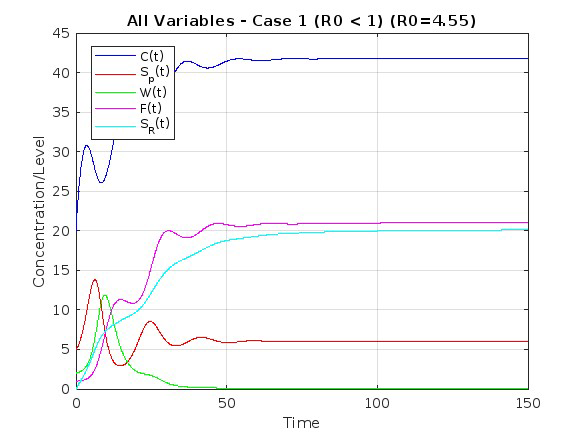
\includegraphics[width=4in,keepaspectratio]{media/fig1.png}
\caption{Simulated time evolution of all state variables for the fractional-order pollution model with \(\alpha = 0.95\) and \(R_{0} = 4.55\). Initial conditions were \(\left( C(0),S_{p}(0),W(0),F(0),S_{R}(0) \right) = (30,2,1,0.5,0)\). The graph shows that all variables approach positive steady-state values (\(C^{*},S_{p}^{*},W^{*},F^{*},S_{R}^{*}\)), confirming the theoretical prediction of global asymptotic stability of the endemic equilibrium \(E^{*}\) for \(R_{0} > 1\).}
\label{fig:all}
\end{figure}

To further analyze the system's behavior, we examine the dynamics of each compartment individually.

\begin{figure}[H]
\centering
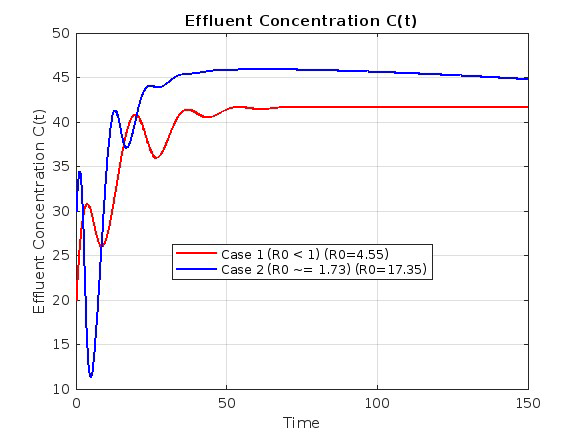
\includegraphics[width=4in,keepaspectratio]{media/fig2.png}
\caption{Simulated dynamics of Effluent Concentration \(C(t)\) for \(R_{0} = 4.55\). The concentration approaches a positive steady-state value \(C^{*}\), distinct from the level \(C_{0} = aN/\Phi_{C}\) associated with the unstable pollution-free equilibrium \(E_{0}\).}
\label{fig:c}
\end{figure}

\begin{figure}[H]
\centering
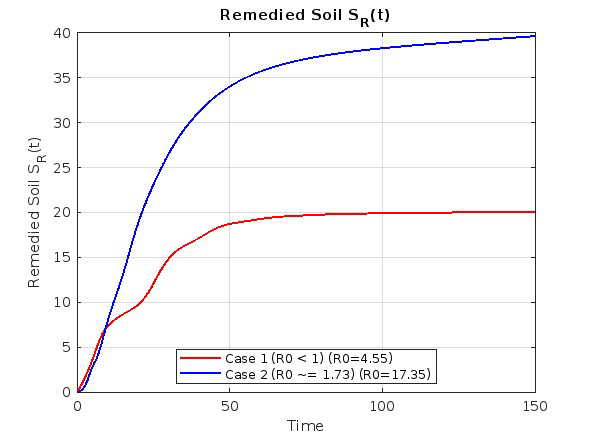
\includegraphics[width=4in,keepaspectratio]{media/fig3.png}
\caption{Simulated dynamics of Polluted Soil \(S_{p}(t)\) for \(R_{0} = 4.55\). The level increases from its initial value and stabilizes at a positive value \(S_{p}^{*}\). This confirms the existence and stability of the endemic equilibrium \(E^{*}\), as \(S_{p}^{*} > 0\) is a defining characteristic.}
\label{fig:sp}
\end{figure}

\begin{figure}[H]
\centering
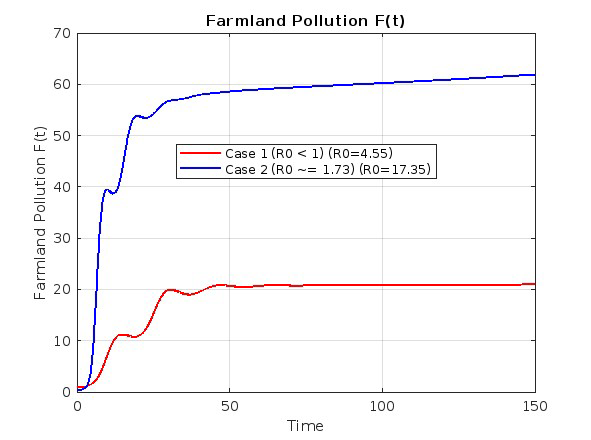
\includegraphics[width=4in,keepaspectratio]{media/fig4.png}
\caption{Simulated dynamics of Water Contamination \(W(t)\) for \(R_{0} = 4.55\). The contamination level rises and approaches a positive steady state \(W^{*}\), indicating that water pollution is sustained rather than eliminated.}
\label{fig:w}
\end{figure}

\begin{figure}[H]
\centering
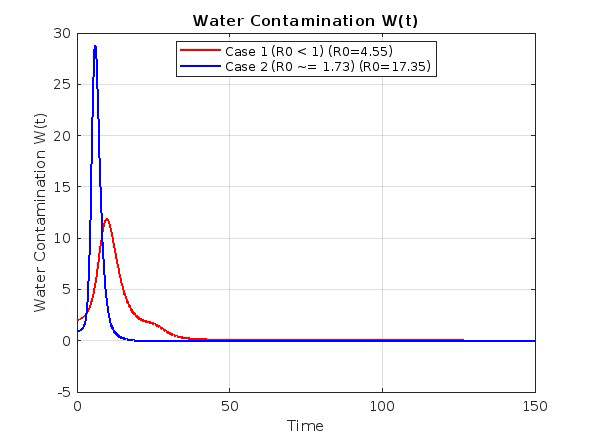
\includegraphics[width=4in,keepaspectratio]{media/fig5.png}
\caption{Simulated dynamics of Farmland Pollution \(F(t)\) for \(R_{0} = 4.55\). The pollution level converges to a positive equilibrium value \(F^{*}\), verifying that \(E^{*}\) is the long-term attractor, with \(F^{*} > 0\), signifying persistent contamination of agricultural land.}
\label{fig:f}
\end{figure}

\begin{figure}[H]
\centering
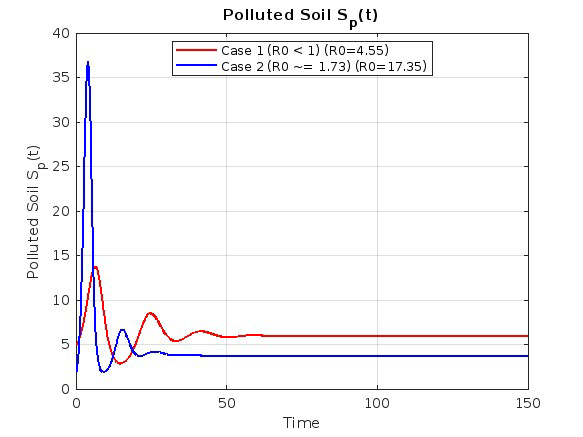
\includegraphics[width=4.in,keepaspectratio]{media/fig6.png}
\caption{Simulated dynamics of Remedied Soil \(S_{R}(t)\) for \(R_{0} = 4.55\). The amount of remediated soil accumulates over time and reaches a steady state \(S_{R}^{*}\). This reflects the balance between ongoing remediation processes (\(\gamma_{1}S_{p}^{*}\), \(\gamma_{2}F^{*}\)) and the degradation rate (\(\Phi_{5}S_{R}^{*}\)) at the stable equilibrium \(E^{*}\).}
\label{fig:sr}
\end{figure}

The numerical simulations for \(R_{0} = 4.55\) provide strong evidence supporting the theoretical stability analysis:

\begin{enumerate}
\def\labelenumi{\arabic{enumi}.}
\item
  \textbf{Effluent Concentration} \(C(t)\) \textbf{(Figure \hyperref[2xcytpi]{2})}: The effluent concentration \(C(t)\) does not settle at the level \(C_{0} = aN/\Phi_{C}\) associated with \(E_{0}\). Instead, it approaches a different positive steady state \(C^{*}\). This deviation from \(C_{0}\) is expected at \(E^{*}\)~due to the active interaction terms (\(- LC^{*}S_{p}^{*}\), \(- BC^{*}W^{*}\)) which are zero at \(E_{0}\)~but non-zero at \(E^{*}\).
\item
  \textbf{Polluted Soil} \(S_{p}(t)\) \textbf{(Figure \hyperref[1ci93xb]{3})}: The level of soil pollution increases from its initial value and stabilizes at a positive value \(S_{p}^{*}\). This is a direct confirmation of the existence and stability of \(E^{*}\), as \(S_{p}^{*} > 0\) is a defining characteristic of the endemic equilibrium. The convergence to \(S_{p}^{*}\) demonstrates that soil pollution becomes persistent in the system when \(R_{0} > 1\).
\item
  \textbf{Water Contamination} \(W(t)\) \textbf{(Figure \hyperref[3whwml4]{4})}: Similarly, the water contamination level \(W(t)\) rises and approaches a positive steady state \(W^{*}\). This behavior aligns with the stability of \(E^{*}\), where \(W^{*} > 0\). It indicates that water pollution is sustained rather than eliminated.
\item
  \textbf{Farmland Pollution} \(F(t)\) \textbf{(Figure \hyperref[qsh70q]{5})}: The farmland pollution level \(F(t)\) also converges to a positive equilibrium value \(F^{*}\). This verifies that \(E^{*}\)~is the long-term attractor, with \(F^{*} > 0\), signifying persistent contamination of agricultural land.
\item
  \textbf{Remedied Soil} \(S_{R}(t)\) \textbf{(Figure \hyperref[3as4poj]{6})}: The amount of remediated soil \(S_{R}(t)\) accumulates over time and reaches a steady state \(S_{R}^{*}\). This reflects the ongoing remediation processes (\(\gamma_{1}S_{p}^{*}\), \(\gamma_{2}F^{*}\)) balancing the degradation rate (\(\Phi_{5}S_{R}^{*}\)) at the stable equilibrium \(E^{*}\). The fact that it reaches a finite value \(S_{R}^{*} = \left( \gamma_{1}S_{p}^{*} + \gamma_{2}F^{*} \right)/\Phi_{5}\) shows that remediation reaches a balance with persistent pollution sources, rather than ceasing.
\end{enumerate}

In summary, the numerical simulations for \(R_{0} = 4.55\) provide strong evidence supporting the theoretical stability analysis. The system's trajectory converges to the unique endemic equilibrium \(E^{*}\), characterized by persistent, non-zero levels of pollution across all active compartments (\(S_{p}^{*},W^{*},F^{*}\)), a corresponding effluent level \(C^{*}\), and a balanced remediation state \(S_{R}^{*}\). This confirms that when \(R_{0} > 1\), the pollution-free state \(E_{0}\)~is unstable, and the system settles into a persistent pollution regime as predicted by the model.

\section{Conclusion}

This study presented a comprehensive analysis of a five-compartment fractional-order model for co-contaminated soil and water pollution dynamics using the Atangana-Baleanu-Caputo derivative. We derived the basic reproduction number \(R_{0}\) as the fundamental threshold parameter governing system behavior:

- When \(R_{0} < \ 1\), the pollution-free equilibrium is globally asymptotically stable and Mittag-Leffler stable, indicating successful pollution elimination

- When \(R_{0} > \ 1\), a unique endemic equilibrium exists and is globally asymptotically stable, predicting persistent pollution across all environmental compartments

As predicted, the pollution-free equilibrium \(E_{0}\) is unstable. Initially polluted compartments (\(S_{p}(t)\), \(W(t)\), \(F(t)\)) approach distinct positive steady-state values (\(S_{p}^{*}\), \(W^{*}\), \(F^{*}\)), indicating persistent pollution. The effluent concentration \(C(t)\) stabilizes at \(C^{*}\), which differs from the level \(C_{0} = aN/\Phi_{C}\) associated with \(E_{0}\). The remediated soil \(S_{R}(t)\) accumulates and reaches a steady state \(S_{R}^{*}\), reflecting a balance between ongoing remediation (\(\gamma_{1}S_{p}^{*}\), \(\gamma_{2}F^{*}\)) and degradation (\(\Phi_{5}S_{R}^{*}\)). This behavior validates the model's prediction of a persistent pollution regime when \(R_{0} > 1\). The system's trajectory converges to \(E^{*}\), characterized by non-zero pollution levels across all active compartments. These results confirm that \(R_{0} = 4.55\) leads to a stable, persistent pollution state rather than elimination.

Our analysis employed advanced techniques including fractional Lyapunov functionals and Mittag-Leffler stability theory to characterize long-term system behavior precisely. We developed an adaptive predictor-corrector numerical scheme specifically tailored for ABC fractional systems, enabling accurate long-term simulations.

This work provides crucial analytical and computational tools for understanding complex pollution dynamics in interconnected environmental media. The threshold condition \(R_{0} < \ 1\) offers practical guidance for pollution control strategies: reducing pollutant input rates, enhancing degradation/remediation processes, and limiting transmission between compartments. Future work will explore optimal control strategies for driving \(R_{0}\) below the critical threshold and investigate spatially explicit extensions of the model.

\textbf{CRediT authorship contribution statement:}

\textbf{Priya P. and Roselyn Besi P.} Conceptualization, Methodology, Writing-Original draft, formal analysis, investigation.

Sabarmathi A.: Scrutinized the work.

\textbf{Declaration of Competing interest:}

The authors declare that they have no known competing financial interests or personal relationships that could have appeared to influence the work reported in this paper.

\textbf{Data Availability:}

Data will be provided by corresponding author on reasonable request.

\textbf{Funding:}

No Funding

\begin{thebibliography}{99}

\bibitem{aty1} Abdel-Aty, M., Abdel-Khalek, S., Obada, A.-S.F.
Pancharatnam phase of two-mode optical fields with Kerr nonlinearity, Optical Review, 2000, 7(6), pp. 499--504 DOI: \url{http://dx.doi.org/10.1007/s10043-000-0499-6}

\bibitem{aty2} Rehman, H.U., Said, G.S., Amer, A., Elazab, N.S., Osman, M.S.
Unraveling the (4+1)-dimensional Davey-Stewartson-Kadomtsev-Petviashvili equation: Exploring soliton solutions via multiple techniques, Alexandria Engineering Journal, 2024, 90, pp. 17--23 DOI: \url{http://dx.doi.org/10.1016/j.aej.2024.01.058}

\bibitem{aty3} Abdel-aty, M.
Quantum field entropy and entanglement of a three-level atom two-mode system with an arbitrary nonlinear medium, Journal of Modern Optics, 2003, 50(2), pp. 161--177 DOI: \url{http://dx.doi.org/10.1080/09500340308235167}

\bibitem{aty4} El-Shahat, T.M., Abdel-Khalek, S., Abdel-Aty, M., Obada, A.-S.F.
Aspects on entropy squeezing of a two-level atom in a squeezed vacuum, Chaos Solitons and Fractals, 2003, 18(2), pp. 289--298 DOI: \url{http://dx.doi.org/10.1016/S0960-0779(02)00652-5}

\bibitem{aty5} Obada, A.-S.F., Abdel-Aty, M.
Influence of the stark shift and kerr-like medium on the evolution of field entropy and entanglement in two-photon processes, Acta Physica Polonica B, 2000, 31(3), pp. 589--599 URL: \url{https://www.actaphys.uj.edu.pl/fulltext?series=Reg&vol=31&page=589}

\bibitem{aty6} Abdel-Aty, M., Abdalla, M.S., Obada, A.-S.F.
Entropy and phase properties of isotropic coupled oscillators interacting with a single atom: one- and two-photon processes, Journal of Optics B Quantum and Semiclassical Optics, 2002, 4(3), pp. S133--S141 DOI: \url{http://dx.doi.org/10.1088/1464-4266/4/3/367}

\bibitem{aty7} Zhang, J.-S., Chen, A.-X., Abdel-Aty, M.
Two atoms in dissipative cavities in dispersive limit: Entanglement sudden death and long-lived entanglement, Journal of Physics B Atomic Molecular and Optical Physics, 2010, 43(2), 025501 DOI: \url{http://dx.doi.org/10.1088/0953-4075/43/2/025501}

\bibitem{aty8} Sebawe Abdalla, M., Hassan, S.S., Abdel-Aty, M.
Entropic uncertainty in the Jaynes-Cummings model in presence of a second harmonic generation, Optics Communications, 2005, 244(1-6), pp. 431--443 DOI: \url{http://dx.doi.org/10.1016/j.optcom.2004.09.051}

\bibitem{aty9} Abdel-Aty, M.
An investigation of entanglement and quasiprobability distribution in a generalized Jaynes-Cummings model, Journal of Mathematical Physics, 2003, 44(4), pp. 1457--1471 DOI: \url{http://dx.doi.org/10.1063/1.1559643}

\bibitem{aty10} Abdel-Aty, M., Sebawe Abdalla, M., Obada, A.-S.F.
Entropy squeezing of a two-mode multiphoton Jaynes-Cummings model in the presence of a nonlinear medium, Journal of Optics B Quantum and Semiclassical Optics, 2002, 4(2), pp. 134--142 DOI: \url{http://dx.doi.org/10.1088/1464-4266/4/2/309}

\bibitem{ref1}
Atangana, A., \& Baleanu, D. (2017). New fractional derivatives with nonlocal and non-singular kernel: Theory and application to heat transfer model. \emph{Thermal Science}, 21(1), 1-7. DOI: \url{https://doi.org/10.2298/TSCI160111018A}

\bibitem{ref2}
Area, I., Batarfi, H., Losada, J., Nieto, J. J., Shammakh, W., \& Torres, A. (2015). On a fractional order Ebola epidemic model. \emph{Advances in Difference Equations}, 2015(1), 278. DOI: \url{https://doi.org/10.1186/s13662-015-0613-5}

\bibitem{ref3}
Diethelm, K. (2010). \emph{The analysis of fractional differential equations: An application-oriented exposition using differential operators of Caputo type}. Springer Science \& Business Media. DOI: \url{https://doi.org/10.1007/978-3-642-14574-2}

\bibitem{ref4}
Deeksha Singh, Farheen Sultana, Rajesh K. Pandey, "Approximation of Caputo-Prabhakar derivative with application in solving time fractional advection-diffusion equation", 2022, \url{https://doi.org/10.1002/fld.5077}.

\bibitem{ref5}
Swati Yadav, Rajesh K. Pandey, Anil K. Shukla," Numerical approximations of Atangana--Baleanu Caputo derivative and its application", Chaos, Solitons \& Fractals, Volume 118, 2019, Pages 58-64, ISSN 0960-0779, \url{https://doi.org/10.1016/j.chaos.2018.11.009}.

\bibitem{ref6}
Baleanu, D., Diethelm, K., Scalas, E., \& Trujillo, J. J. (2019). \emph{Fractional calculus: models and numerical methods} (Vol. 5). World Scientific. DOI: \url{https://doi.org/10.1142/10044}

\bibitem{ref7}
Li, C., \& Zhang, F. (2019). A survey on the stability of fractional differential equations. \emph{The European Physical Journal Special Topics}, 228(1), 73-84. DOI: \url{https://doi.org/10.1140/epjst/e2011-01379-1}

\bibitem{ref8}
Vargas-De-Le\'{o}n, C. (2012). Volterra-type Lyapunov functions for fractional-order epidemic systems. \emph{Communications in Nonlinear Science and Numerical Simulation}, 17(9), 3617-3622. DOI: \url{https://doi.org/10.1016/j.cnsns.2011.12.014}

\bibitem{ref9}
Baleanu, D., Machado, J. A. T., \& Luo, A. C. J. (Eds.). (2012). \emph{Fractional dynamics and control}. Springer Science \& Business Media. DOI: \url{https://doi.org/10.1007/978-1-4614-0457-6}

\bibitem{ref10}
Pagnini, G. (2019). Erd\'{e}lyi-Kober fractional diffusion. In \emph{Handbook of Fractional Calculus with Applications} (pp. 265-280). De Gruyter. DOI: \url{https://doi.org/10.1515/9783110571660-011}

\bibitem{ref11}
Sheikh, N. A., Dennis, L. C. C., Ijarola, O. A., Zainal, A. A., \& Mohamad, M. (2022). A review of the developments in the field of fractional calculus and its applications. \emph{Alexandria Engineering Journal}, 61(12), 10137-10153. DOI: \url{https://doi.org/10.1016/j.aej.2022.03.045}

\bibitem{ref12}
Singh, D., Sultana, F., Pandey, R.K. et al. A comparative study of three numerical schemes for solving Atangana--Baleanu fractional integro-differential equation defined in Caputo sense. Engineering with Computers 38 (Suppl 1), 149--168 (2022). DOI: \url{https://doi.org/10.1007/s00366-020-01132-6}

\bibitem{ref13}
Atangana, A., \& Algahtani, O. J. J. (2015). Extension of the groundwater flow model to the concept of fractional variable order derivative. \emph{Abstract and Applied Analysis}, 2015. DOI: \url{https://doi.org/10.1155/2015/341258}

\bibitem{ref14}
Sun, H., Chang, A., Zhang, Y., \& Chen, W. (2019). Modeling anomalous heat transport in geothermal reservoirs via fractional Laplacian. \emph{International Journal of Numerical and Analytical Methods in Geomechanics}, 43(14), 2327-2342. DOI: \url{https://doi.org/10.1002/nag.2974}

\bibitem{ref15}
Sardanyes, J., Farner, S., \& Alsed\`{a}, L. (2022). Bifurcations and long-term dynamics in a discrete ecological model with fractional-order recurrences. \emph{Chaos, Solitons \& Fractals}, 154, 111654. DOI: \url{https://doi.org/10.1016/j.chaos.2021.111654}

\bibitem{ref16}
Swati Yadav, Rajesh K. Pandey," Numerical approximation of fractional burgers equation with Atangana--Baleanu derivative in Caputo sense", Chaos, Solitons \& Fractals, Volume 133, 2020, 109630, ISSN 0960-0779. DOI: \url{https://doi.org/10.1016/j.chaos.2020.109630}

\end{thebibliography}

\end{document}
